%!TEX root = ../lections.tex
Под многомерными динамическими системами понимаются системы, размерность фазового пространства которых равна трем и выше. 
\begin{wrapfigure}[9]{l}{0.75\linewidth} 
	\vspace{0.1em}
	\centering
	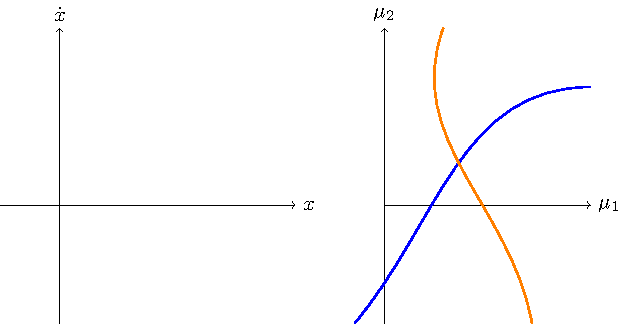
\includegraphics[scale=1]{fig/fig48.pdf}
	\vspace{-0.25em}
\end{wrapfigure}
Для систем на плоскости задача была разбить плоскость параметров на области с разными характеристическими бифуркационными линиями.

На фазовой плоскости существовало конечное число предельных циклов и состояний равновесия.

Многомерные системы делятся на 2 класса:
\begin{enumerate}
	\item Системы с конечным числом состояний равновесия, периодических движений и числом бифуркаций. Такие системы носят название систем Морса-Смейла. Они есть подобие двумерных систем.
	\item Системы с бесконечным числом периодических движений и бифуркаций. 
\end{enumerate}

Интересны бифуркации, при которых один класс переходит в другой.

\subsection{Основные бифуркации состояний равновесия трехмерных систем}
Запишем систему:
\begin{equation}
	\begin{cases}
		\dot x = P(x, y, z, \mu) \\
		\dot y = Q(x, y, z, \mu) \\
		\dot z = R(x, y, z, \mu),
	\end{cases}
	\label{eq:107}	
\end{equation}

Без ограничения общности, будем считать, что состояние равновесия в начале координат $O_0(x=y=z=\mu=0),~\mu \in [-\mu_0,\mu_0]$.

\textit{Двукратное равновесие:}

$\lambda_1(0)=0,~Re[\lambda_{2,3}(\mu)] \neq 0$

Перепишем, приведя систему к нормальному виду:
\begin{gather*}
	\dot U_1 = \mu+lU_1^2+\dots, \\
	\dot V=\beta(\mu)V+\dots, \\
	V=
	\begin{pmatrix}
		U_2 \\
		U_3
	\end{pmatrix}
	.
\end{gather*}

\underline{Случай а:}
\begin{gather*}
	\beta(\mu)=
	\begin{pmatrix}
		\lambda_2~~0 \\
		0~~\lambda_3
	\end{pmatrix}
	.
\end{gather*}

Случай аналогичен седлоузлу в двумерной системе. Условие невырожденности: $l\neq 0$,
\begin{gather*}
	\beta(\mu)=
	\begin{cases}
		\dot U_1 = \mu+lU_1^2+\dots \\
		\dot U_2 = \lambda_2U_2+\dots \\
		\dot U_3 = \lambda_3U_3+\dots.
	\end{cases}
\end{gather*}

Пусть $\lambda_2,~\lambda_3<0,~l>0,~U_1^2=-\frac{\mu}{l}$:
\begin{figure}[H]
	\centering
	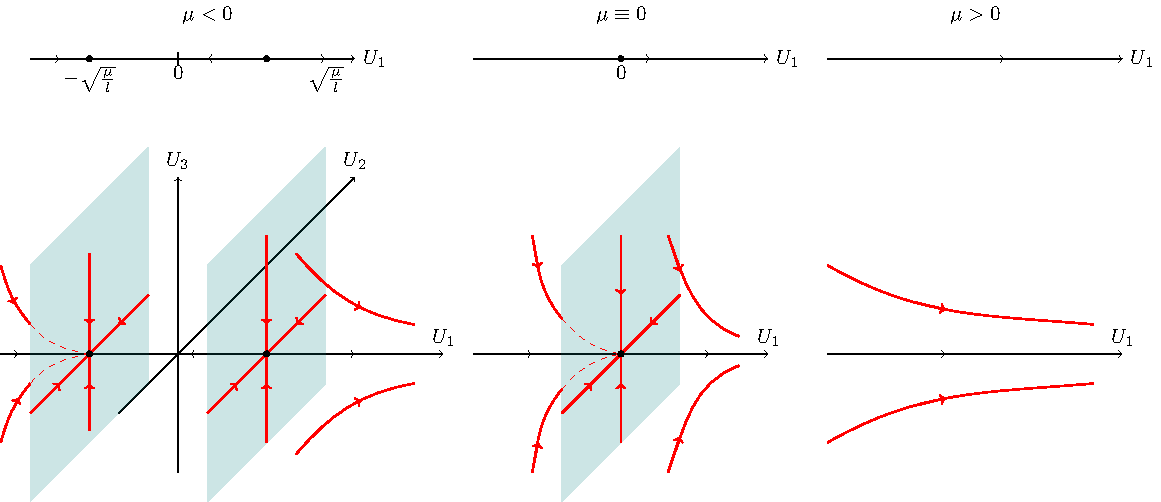
\includegraphics[width=1\linewidth]{fig/fig49.pdf}   
\end{figure}

При $\mu<0$ - устойчивый узел и седло с одномерной сепаратрисой. При $\mu=0$ седлоузел - негрубое состояние равновесия, которое при изменении параметра либо распадается на два, либо исчезает. 

\underline{Случай b:}
\begin{gather*}
	\lambda_{2,3}=\alpha(\mu)\pm i \beta(\mu), \\
	\beta(\mu)=
	\begin{pmatrix}
		\alpha~~-\beta \\
		\beta~~~~\alpha
	\end{pmatrix}
	.
\end{gather*}

Предполагаем, что $Re[\alpha(\mu)]<0$.
\begin{gather*}
	\beta(\mu)=
	\begin{cases}
		\dot U_1 = \mu+lU_1^2+\dots \\
		\dot U_2 = \alpha U_2-\beta U_3 \\
		\dot U_3 = \beta U_2+\alpha U_3.
	\end{cases}
\end{gather*}
\begin{figure}[H]
	\centering
	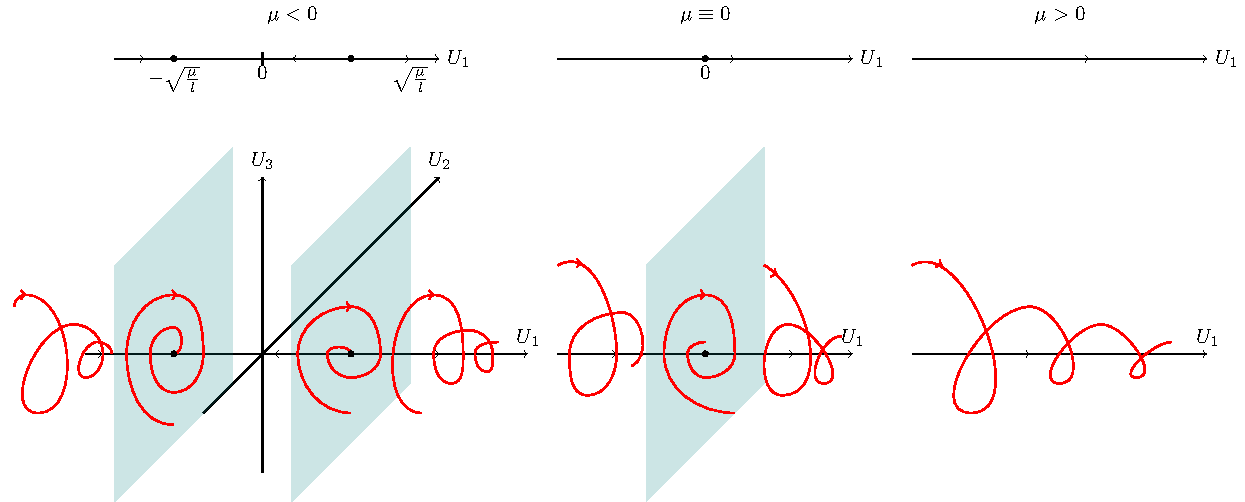
\includegraphics[width=1\linewidth]{fig/fig50.pdf}   
\end{figure}

При $\mu<0$ - устойчивый фокус и седлофокус. При $\mu=0$ седлофокус-фокус.

Пусть корни все действительные. $\lambda_3<0,~\lambda_2>0,~\mu<0$. Для удобства расположим оси координат следующим образом:
\begin{wrapfigure}[6]{l}{0.5\linewidth} 
	\vspace{0.1em}
	\centering
	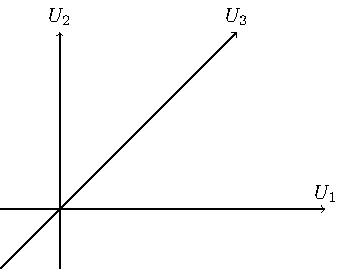
\includegraphics[scale=1]{fig/fig51.pdf}
	\vspace{-0.25em}
\end{wrapfigure}

Одно седло имеет одномерную сепаратрису и двумерное устойчивое многообразие, другое - одно неустойчивое двумерное многообразие и устойчивое одномерное.

\begin{figure}[H]
	\centering
	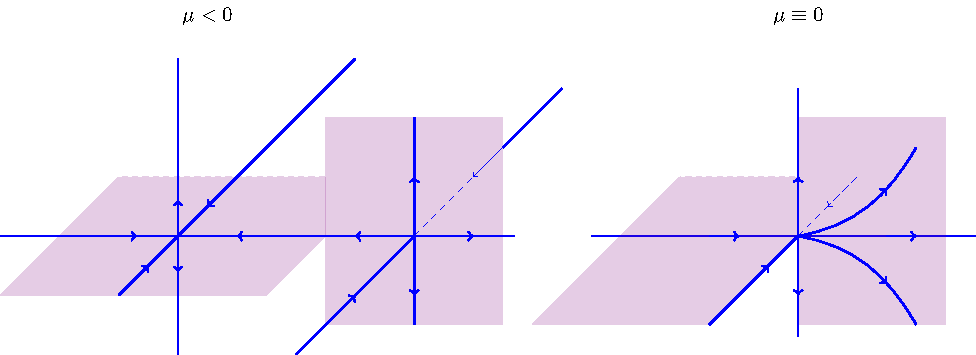
\includegraphics[width=1\linewidth]{fig/fig52.pdf}   
\end{figure}

Многообразия пересекаются, сближаются. Образуется точка, которая при $\mu>0$ исчезает.

27.05
\subsection{Бифуркация коразмерности 1 Андронова-Хопфа}
Предположим, есть состояние равновесия. Его корни комплексно-сопряженные: $\lambda_{1,2}=\alpha(\mu)\pm i \beta(\mu),~\beta(\mu)>0,~\mu=0$ - бифуркационный параметр, который состоит в том, что $\alpha(0)=0$. Условие невырожденности - первая ляпуновская величина $L(\mu)\neq 0$.

Рассмотрим конкретный вид зависимости:
\begin{wrapfigure}[7]{l}{0.42\linewidth} 
	\vspace{0.1em}
	\centering
	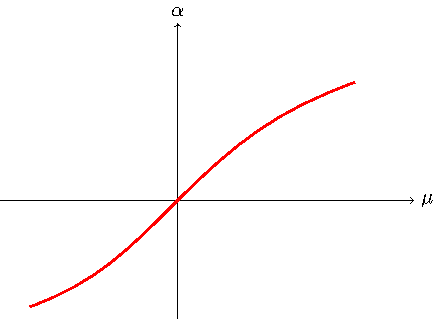
\includegraphics[scale=1]{fig/fig53.pdf}
	\vspace{-0.25em}
\end{wrapfigure}

$\lambda_3(\mu)\neq 0,~L(\mu)<0$,
\begin{equation}
	\begin{cases}
		\dot U_1 = \alpha(\mu)U_1-\beta(\mu)U_2+L(\mu)(U_1^2+U_2^2)U_1+\dots \\
		\dot U_2 = \beta(\mu)U_1+\alpha(\mu)U_2+L(\mu)(U_1^2+U_2^2)U_2+\dots \\
		\dot U_3 = \lambda_3(\mu)U_3+\dots
	\end{cases}
	\label{eq:108}	
\end{equation}

 Для определенности $\lambda_3(\mu)<0$ (рассмотреть $\lambda_3(\mu)>0$).

 Фактически, для рассмотрения такой системы нам достаточно знаний о двумерных системах. Из третьего уравнения системы находим, что $U_3=0$ - инвариантная плоскость. Без третьего уравнения остается двумерная система. Легко восстановить фазовые портреты:
 \begin{figure}[H]
	\centering
	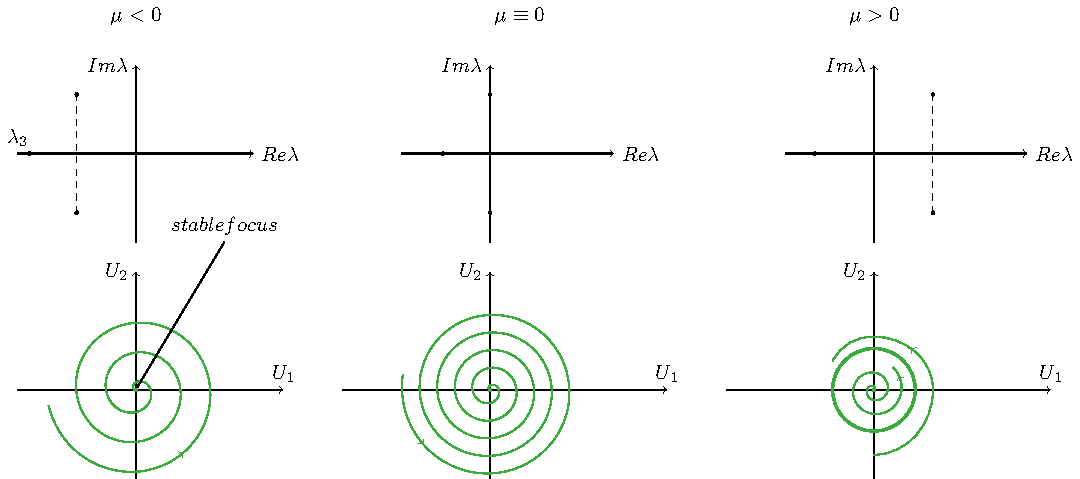
\includegraphics[width=1\linewidth]{fig/fig54.pdf}   
\end{figure}

При $\mu=0$ состояние равновесия не центр, а сложный устойчивый фокус. В этом случае динамику системы определяют кубические слагаемые. При $\mu>0$ появляется предельный устойчивый цикл. 

$\lambda_3<0,~U_3 \rightarrow 0$. $U_3$ - устойчивая плоскость (если рассмотреть одномерную систему на прямой).

\begin{center}
    \begin{minipage}{0.32\linewidth}
        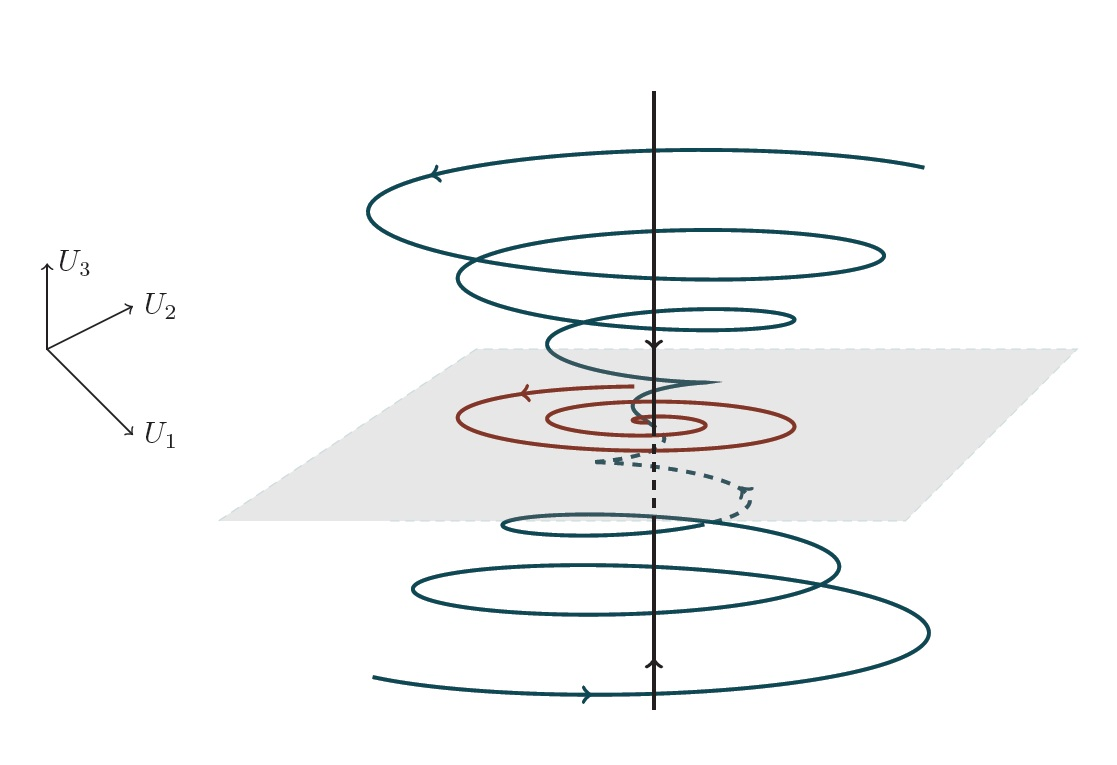
\includegraphics[width=\linewidth]{fig/55_1.jpg} 
        \vspace{-50pt}
        \label{fig:1}
    \end{minipage}
\hfill     
    \begin{minipage}{0.3\linewidth}
        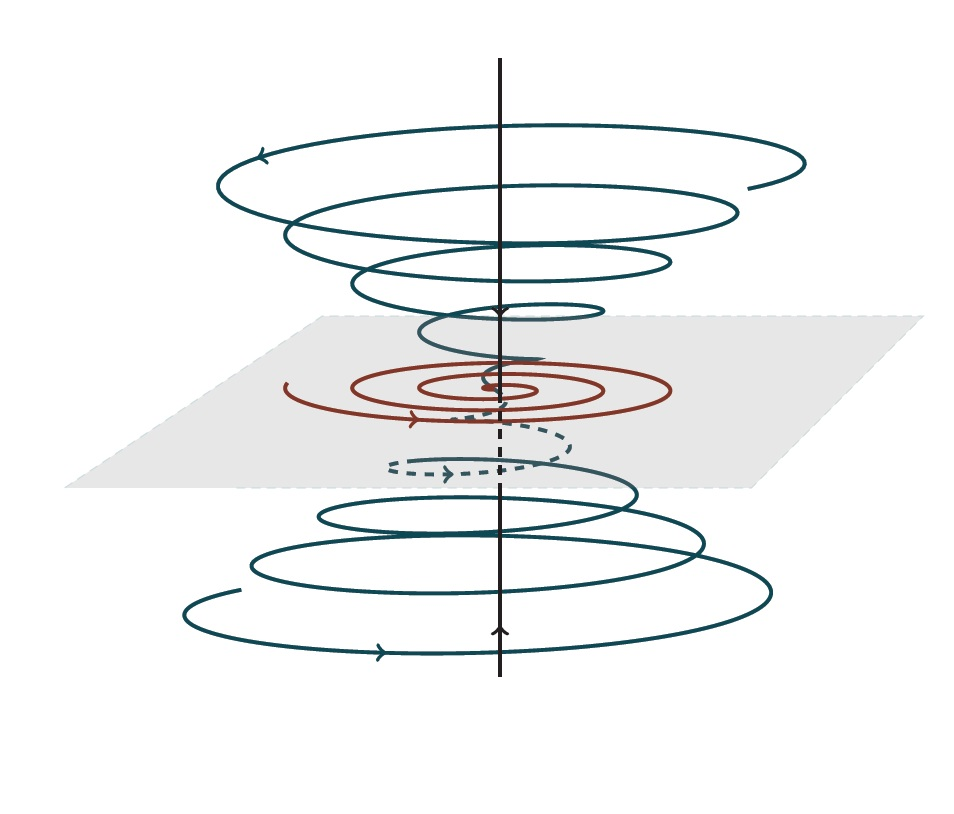
\includegraphics[width=\linewidth]{fig/55_2.jpg} 
        \vspace{-50pt}
        \label{fig:1}
    \end{minipage}
\hfill     
    \begin{minipage}{0.3\linewidth}
        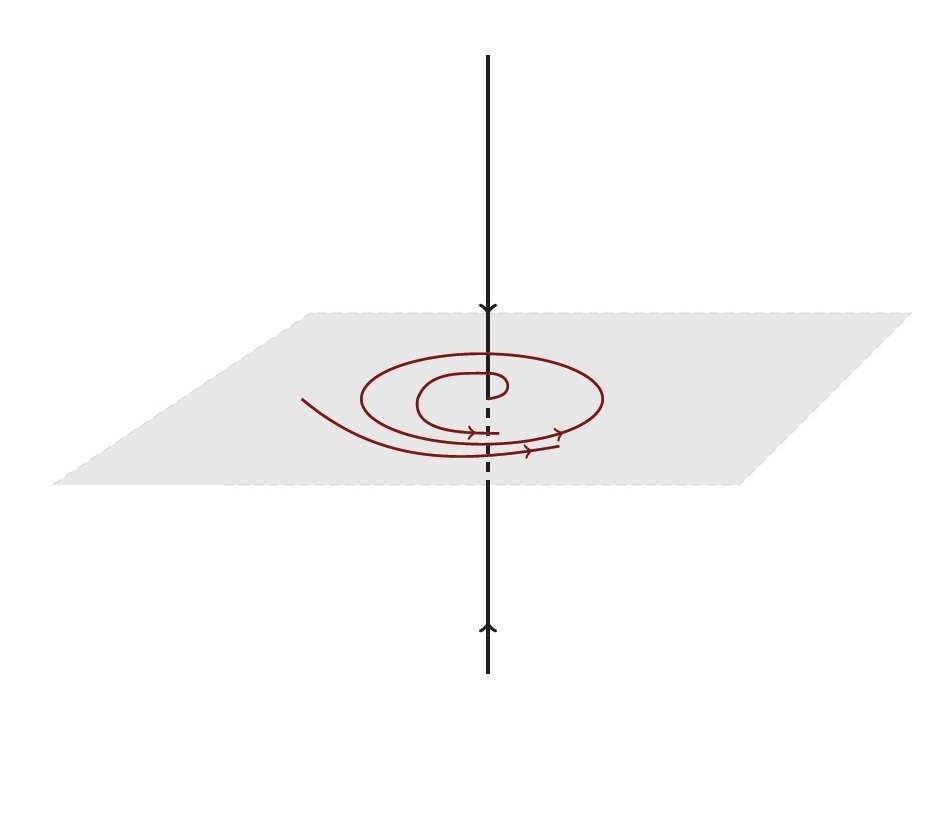
\includegraphics[width=\linewidth]{fig/55_3.jpg} 
        \vspace{-50pt}
        \label{fig:1}
    \end{minipage}    
\end{center}

Справа - неустойчивый седлофокус.

$L>0:$
\begin{figure}[H]
	\centering
	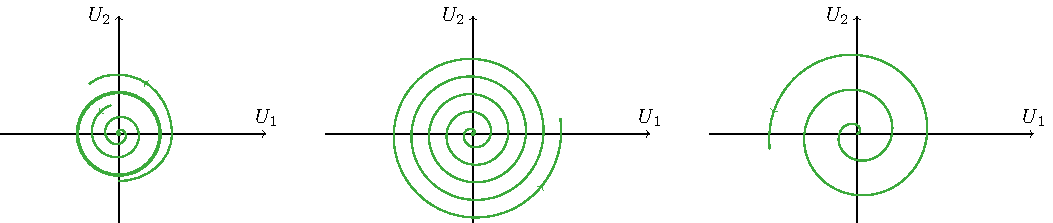
\includegraphics[width=1\linewidth]{fig/fig58.pdf}   
\end{figure}

\begin{center}
    \begin{minipage}{0.32\linewidth}
        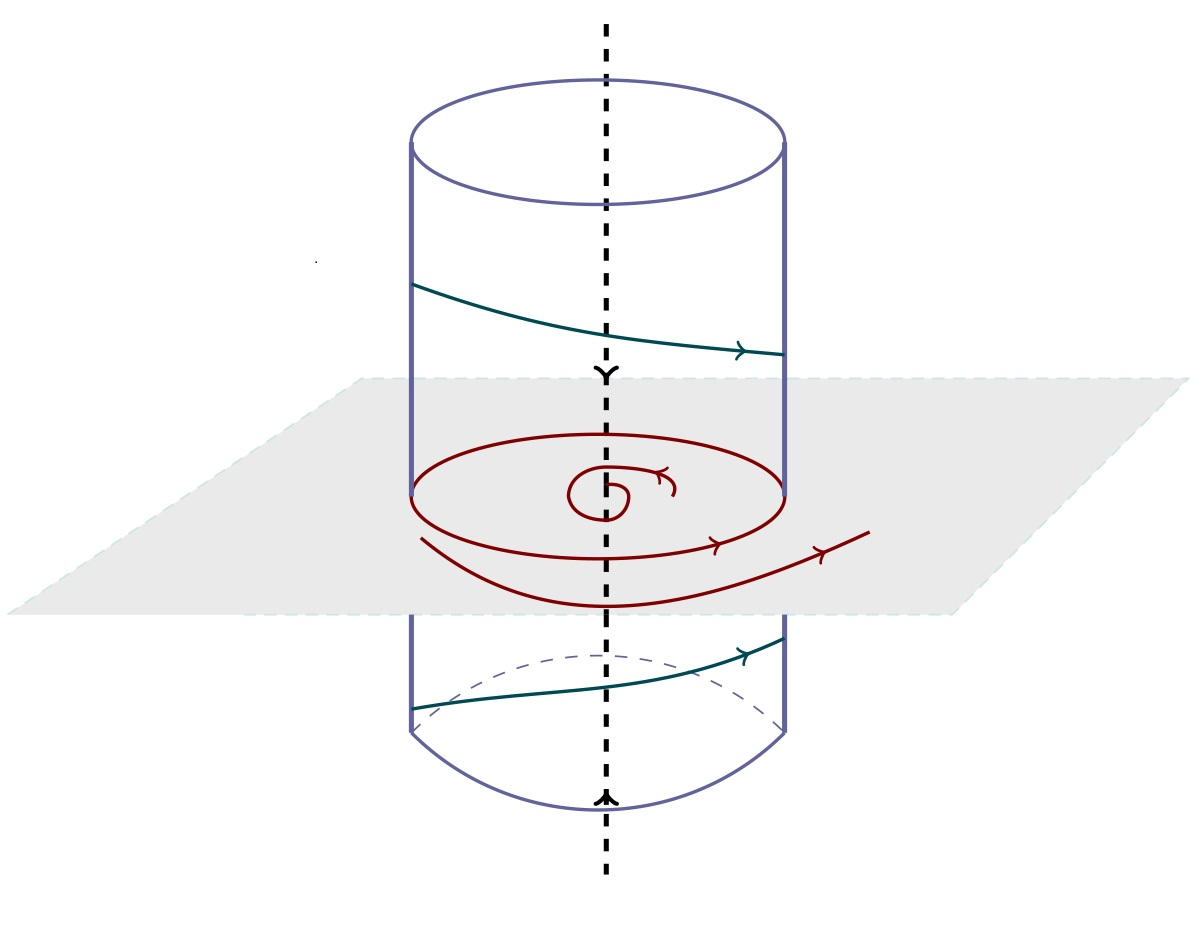
\includegraphics[width=\linewidth]{fig/fig61.jpg} 
        \vspace{-50pt}
        \label{fig:1}
    \end{minipage}
\hfill     
    \begin{minipage}{0.3\linewidth}
        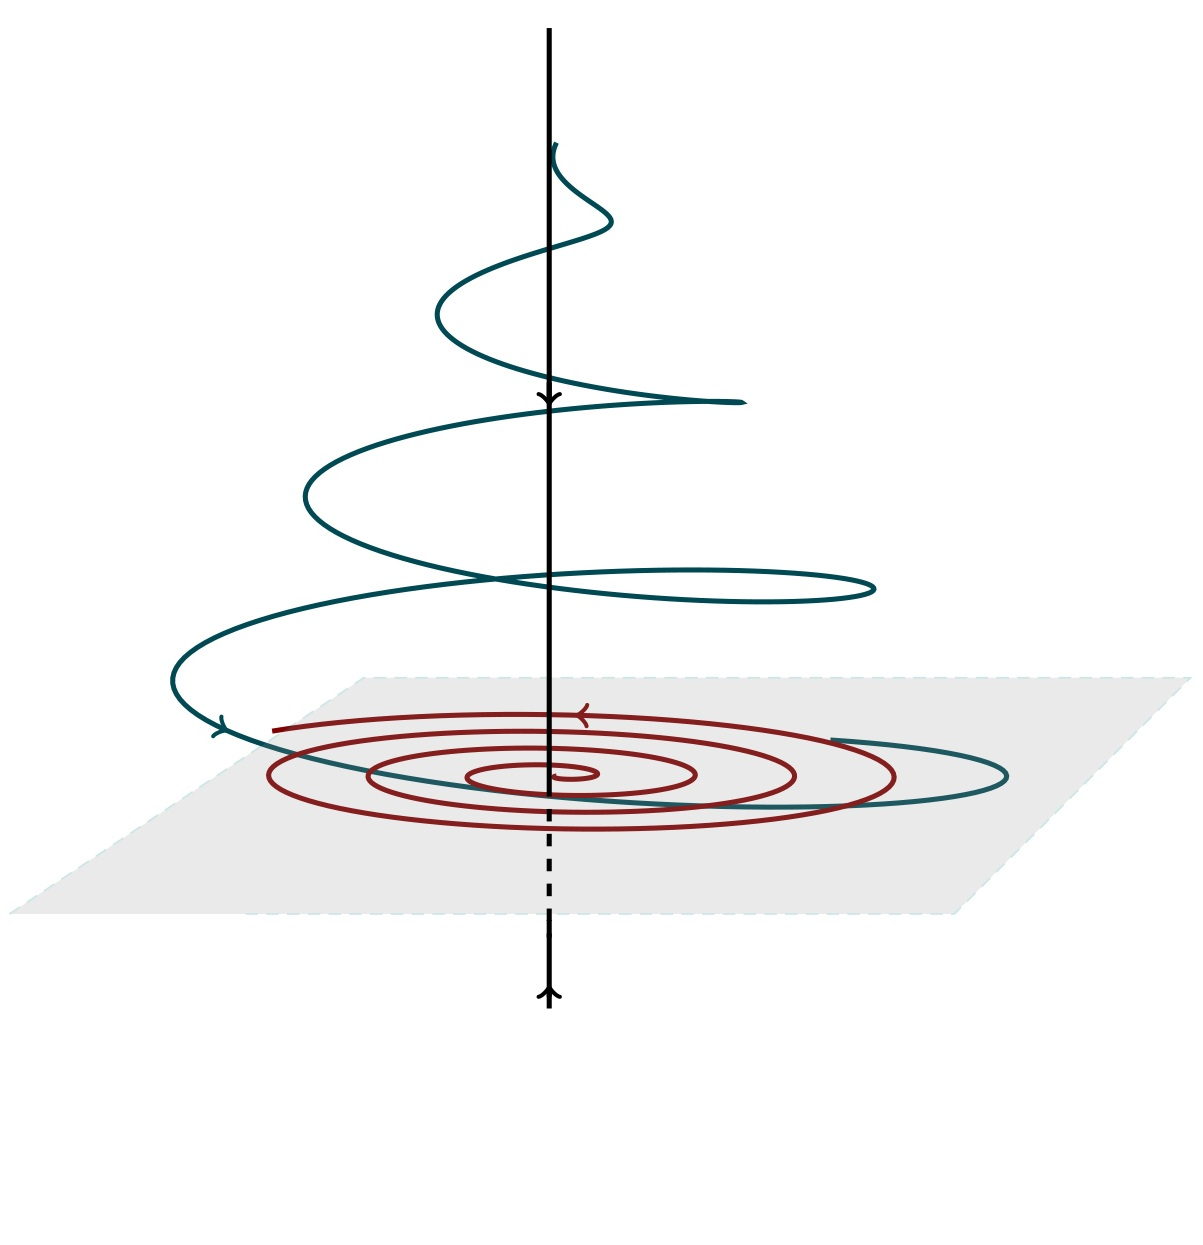
\includegraphics[width=\linewidth]{fig/fig60.jpg} 
        \vspace{-50pt}
        \label{fig:1}
    \end{minipage}
\hfill     
    \begin{minipage}{0.3\linewidth}
        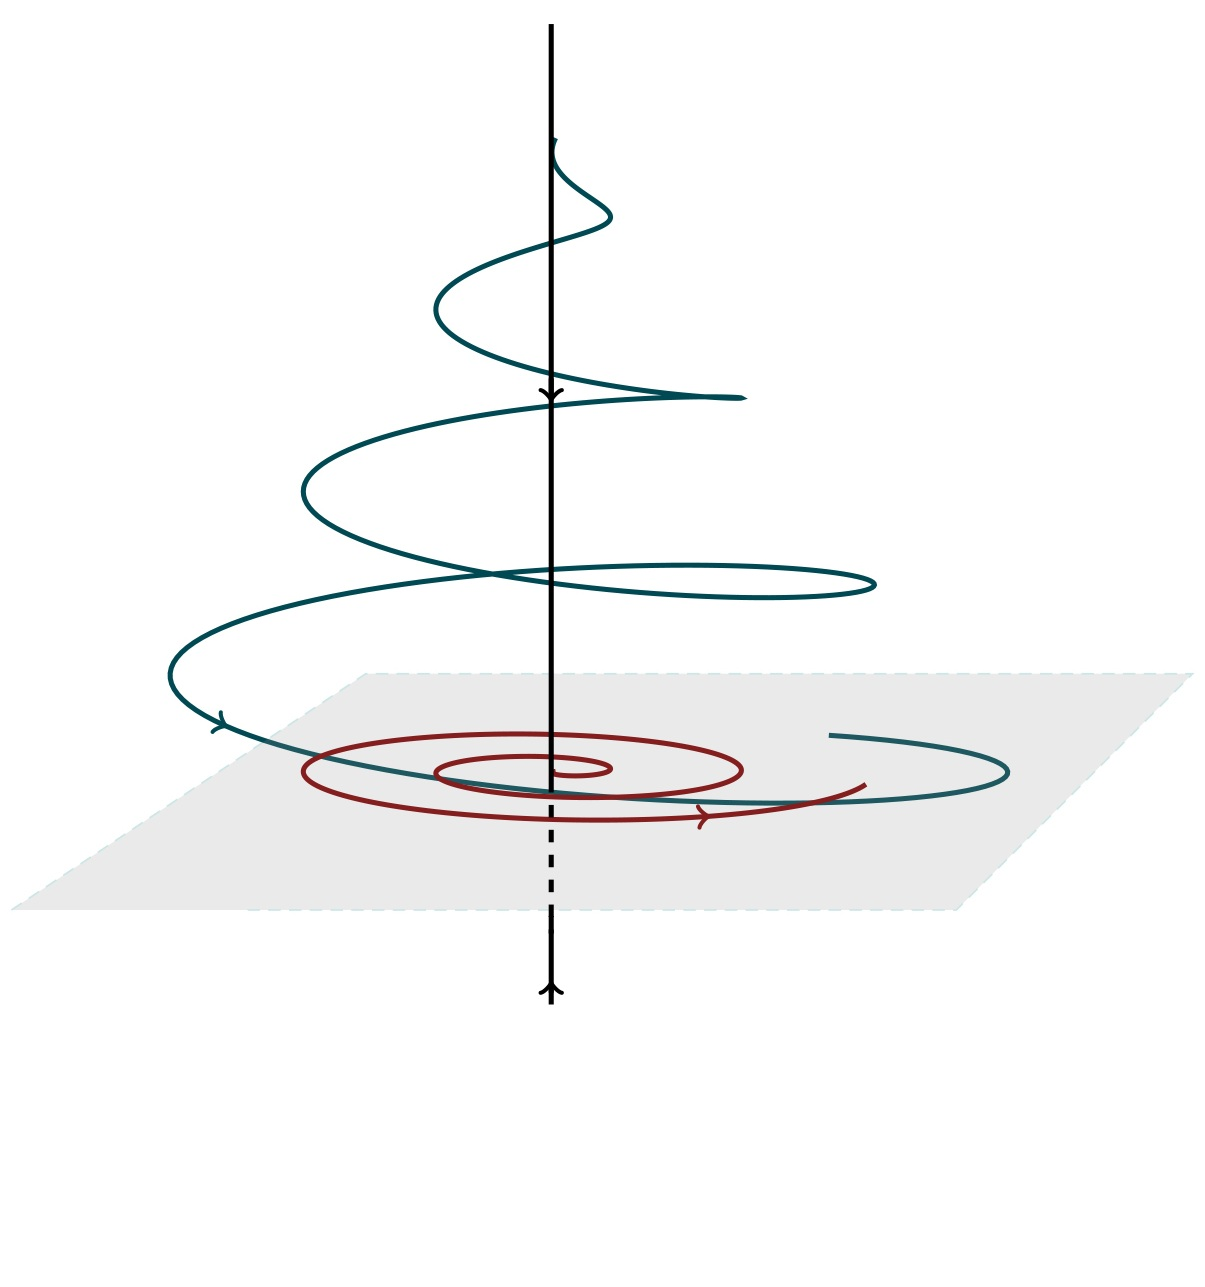
\includegraphics[width=\linewidth]{fig/fig59.jpg} 
        \vspace{-50pt}
        \label{fig:1}
    \end{minipage}    
\end{center}

Слева седловой предельный цикл, по центру - точка стала неустойчивым сложным фокусом.

\subsection{Бифуркации периодических движений в трехмерном пространстве(бифуркация +1)}
Предположим, есть система третьего порядка, в которой существует предельный цикл $L_{\mu}$, зависящий от $\mu$. Для введения мультипликатора выберем произвольную точку, через нее проведем секущую Пуанкаре. Мультипликаторов три, один из которых тривиальный: $s_1(\mu),~s_2(\mu)$.
\begin{wrapfigure}[7]{l}{0.6\linewidth} 
	\vspace{0.1em}
	\centering
	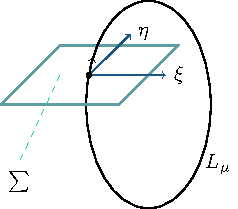
\includegraphics[scale=1]{fig/fig62.pdf}
	\vspace{-0.25em}
\end{wrapfigure}

Первое - седло-узловая бифуркация предельных циклов (двукратный предельный цикл). Предположим, $s_j(\mu)>0$, и при $\mu<0$ оба мультипликатора расположены внутри единичной окружности. При этом $0<s_2(\mu)<1$.
\begin{figure}[H]
	\centering
	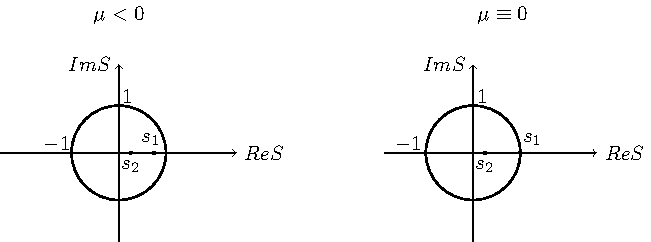
\includegraphics[width=1\linewidth]{fig/fig63.pdf}   
\end{figure}

При $\mu=0: s_1(0)= 1$. Запишем нормальную форму для этой бифуркации. На секущей Пуанкаре вводятся координаты. Тогда поведение вблизи $L_{\mu}$ может быть описано двумерным отображением:
\begin{equation}
	\begin{cases}
		\stackrel{\_}{\xi}= \mu+\xi+\xi^2+\dots \equiv g\\
		\stackrel{\_}{\eta}= s_2(\mu)\eta+\dots
	\end{cases}
	\label{eq:109}	
\end{equation}

Переменные $\xi, \eta$ вводятся в малой $\varepsilon$-окрестности предельного цикла. $\mu$ близко к 0.

g может быть исследовано независимо. Неподвижные точки $\stackrel{\_}{\xi}=\xi$:
$$\xi^2+\mu=0.$$

При $\mu<0: \xi^2=-\mu~\rightarrow \xi=\pm \sqrt{-\mu}$.

Устойчивость:
\begin{gather*}
	g'_{\xi}=1+2\xi, \\
	g''_{\xi \xi}=2,
\end{gather*}
$\xi$ мало, следовательно, $g'_{\xi}>0$. Функция монотонно растет и выпукла вниз.
\begin{figure}[H]
	\centering
	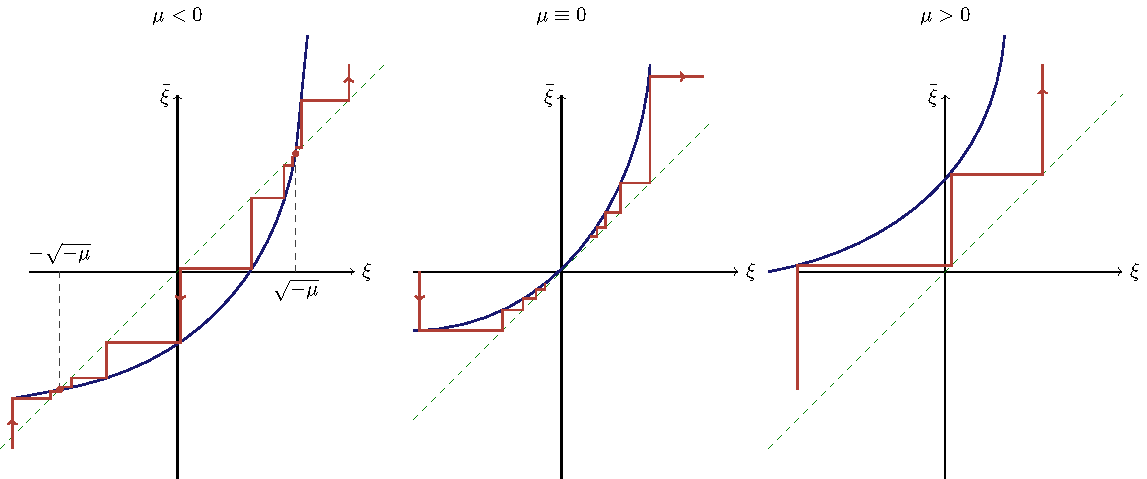
\includegraphics[width=1\linewidth]{fig/fig64.pdf}   
\end{figure}

При $\mu=0 g'=1, s_1=1$ - точка полуустойчивая. 

Из второго уравнения системы получаем, что $\eta=0$ - инвариантная прямая. Любая точка, взятая на этой прямой, перепрыгнет на нее же. Она устойчива:  
\begin{figure}[H]
	\centering
	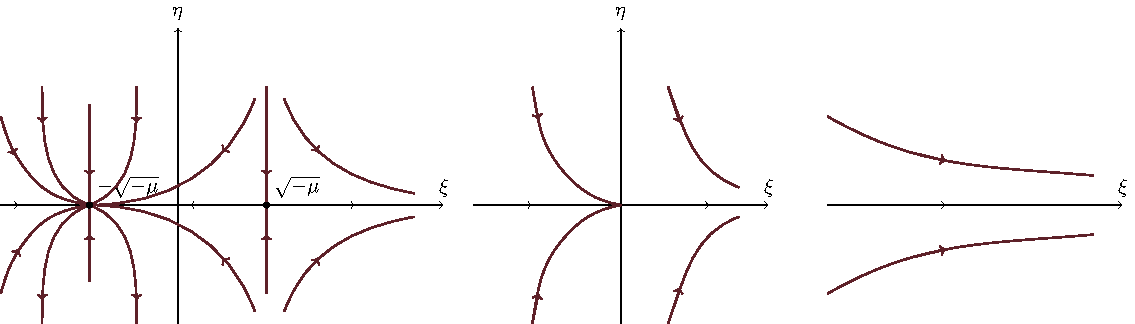
\includegraphics[width=1\linewidth]{fig/fig65.pdf}   
\end{figure}

Слева направо: на вертикальных прямых действует второе отображение. На них траектории стремятся к $\eta=0$. Затем остается одна неподвижная точка - седлоузел (это не равновесие, а отображение). После чего исчезает.

Это все отображения, т.е набор точек (нарисовано сплошными).
\begin{figure}[H]
	\centering
	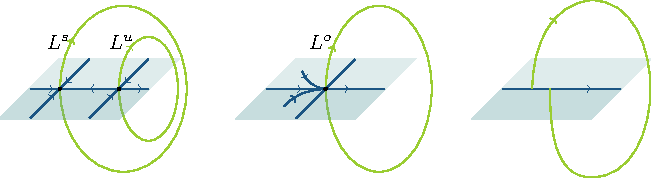
\includegraphics[width=1\linewidth]{fig/fig66.pdf}   
\end{figure}

Слева устойчивый (внешний) и седловой (внутренний) предельные циклы. Им соответствуют неподвижные точки. По центру негрубая неподвижная точка и двукратный предельный цикл. Справа - нет предельного цикла.

\subsection{Бифуркация удвоения периода (бифуркация -1)}
Пусть мультипликаторы отрицательные:
\begin{figure}[H]
	\centering
	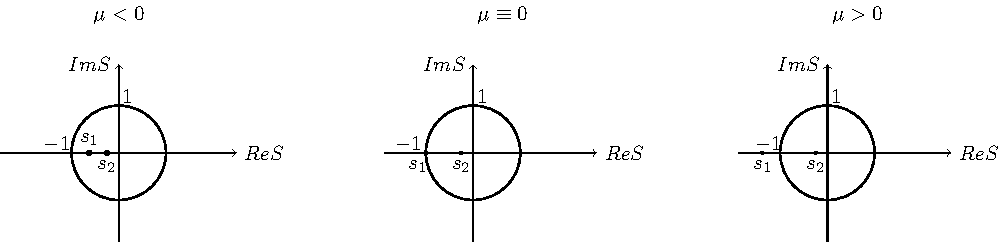
\includegraphics[width=1\linewidth]{fig/fig67.pdf}   
\end{figure}

Динамику поведения в окрестности предельного цикла можно описать нормальной формой:
\begin{equation}
	\begin{cases}
		\stackrel{\_}{\xi}= -(1+\mu)\xi+\xi^3+\dots \equiv g(\xi,\mu)\\
		\stackrel{\_}{\eta}= s_2(\mu)\eta+\dots
	\end{cases}
	\label{eq:110}	
\end{equation}

Первое уравнение можно исследовать отдельно. Мультипликаторы отрицательны, следовательно, будут перескоки. 

Удобнее начать с отображения $\stackrel{=}{\xi}$, т.е. посмотреть, как ведет себя система через две итерации.
\begin{gather*}
	\stackrel{=}{\xi}=-(1+\mu)\stackrel{\_}{\xi}+\stackrel{\_}{\xi}^3+\dots= \\
	=-(1+\mu)(-(1+\mu)\xi+\xi^3)+(-(1+\mu)\xi+\xi^3)^3+\dots= \\
	=(1+\mu)^2\xi-(1+\mu)\xi^3-(1+\mu)^3\xi^3+\dots=(1+\mu)^2\xi-(1+\mu)((1+\mu)^2+1)\xi^3+\dots
\end{gather*}


Найдем неподвижные точки. Есть тривиальная $\xi=0$ -- она устойчива при $\mu<0$,т.к. мультипликатор меньше единицы. При $\mu=0$ мультипликатор равен единице, точка полуустойчава, при $\mu>0$ неустойчива.

Нетривиальные точки:
\begin{gather*}
	1=(1+\mu)^2-(1+\mu)(2+2\mu+\mu^2)\xi^2, \\
	\cancel{1}=\cancel{1} +2\mu+\mu^2-(1+\mu)(2+2\mu+\mu^2)\xi^2, \\
	\xi^2=\frac{\mu(2+\xcancel{\mu)}}{(1+\cancel{\mu})(2+\xcancel{2\mu}+\xcancel{\mu^2})},
\end{gather*}

Вспоминая, что $\mu$ мало и близко к 0:
\begin{gather*}
	\xi^2 \approx \frac{2\mu}{2}=\mu.
\end{gather*}

При $\mu>0$ существует пара неподвижных точек $\xi=\pm \sqrt{\mu}$:
\begin{figure}[H]
	\centering
	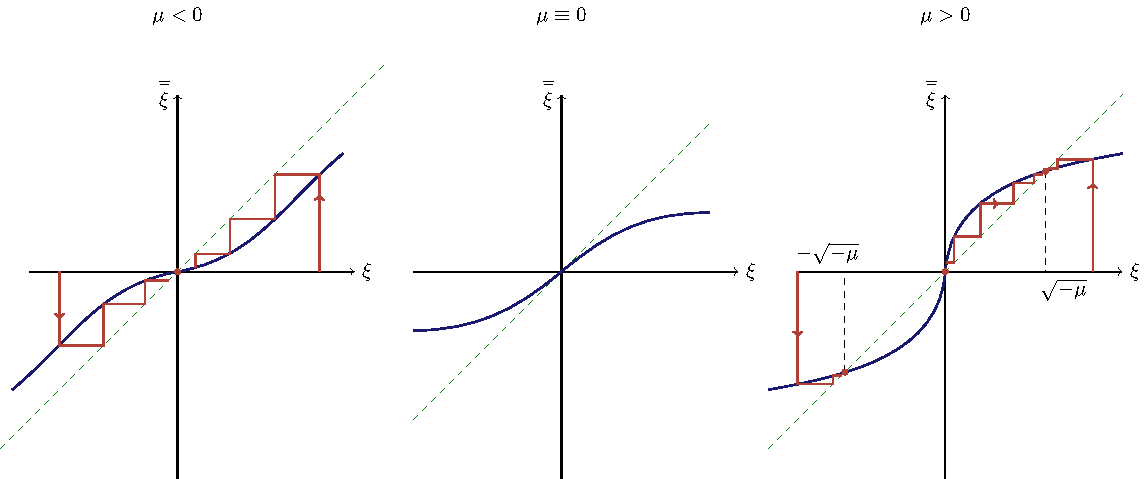
\includegraphics[width=1\linewidth]{fig/fig68.pdf}   
\end{figure}
Слева -- устойчивая точка, по центру -- касание (мультипликатор 1), справа появляются нетривиальные точки.

Если в отображении $g^2$ есть неподвижная точка, то для $g^1$ есть периодическая траектория периода 2.
\begin{figure}[H]
	\centering
	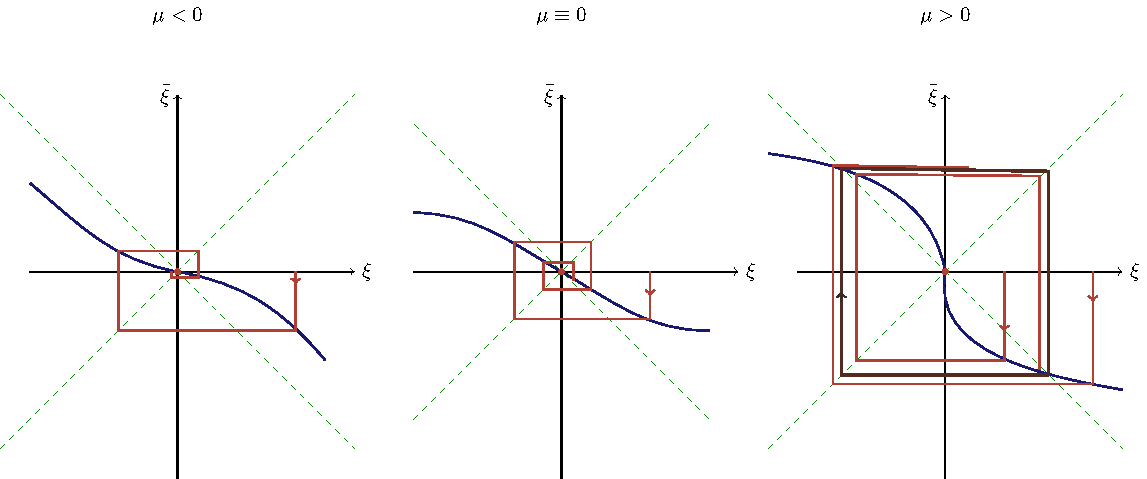
\includegraphics[width=1\linewidth]{fig/fig69.pdf}   
\end{figure}
Синяя - функция последования. Справа -- устойчивая точка с перескоком. По центру -- сложная устойчивая неподвижная точка, траектории близко друг к другу. Справа -- есть периодическая траектория.

В исходной системе (секущая Пуанкаре будет вертикально):
\begin{figure}[H]
	\centering
	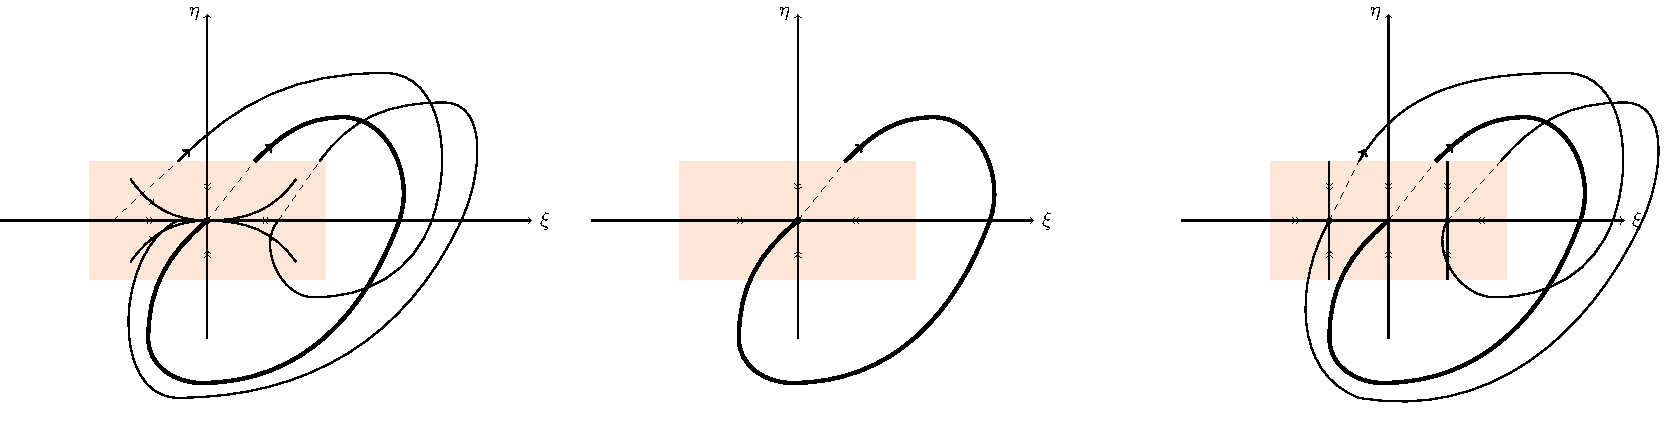
\includegraphics[width=1\linewidth]{fig/fig70.pdf}   
\end{figure}
Слева -- устойчивая неподвижная точка, которой соответствует устойчивый предельный цикл. Неподвижная точка стала седловой, устойчивый предельный цикл стал неустойчивым. Появился новый предельный цикл с удвоенным исходным периодом. 

Был исходный предельный цикл, мы слегка поменяли параметр. Траектория начала промахиваться и замкнулась только на втором обороте. 

\subsection{Бифуркация рождения инвариантного тора}
Пусть есть предельный цикл и
\begin{figure}[H]
	\centering
	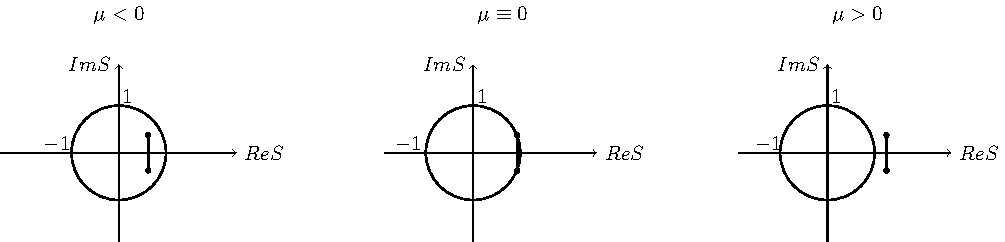
\includegraphics[width=1\linewidth]{fig/fig71.pdf}   
\end{figure}
В момент бифуркации при $\mu=0$ можно записать: $s_{1,2}=e^{\pm i\omega}$, где $\omega \neq 0,\omega \neq \pi$ (такое уже рассмотрели) и $\omega \neq \frac{2\pi}{3},\omega \neq \frac{\pi}{2}$ (резонансны случаи, описывают бифуркации коразмерности 2 и выше).

Отображение Пуанкаре в полярных координатах:
\begin{equation}
	\begin{cases}
		\stackrel{\_}{\rho}= (1+\mu)\rho+G(\mu)\rho^3+\dots \\
		\stackrel{\_}{\theta}= \theta+\omega+B(\mu)\rho^2+\dots
	\end{cases}
	\label{eq:s9:4}	
\end{equation}

Здесь $G(\mu)$ играет роль первой ляпуновской величины. Предполагаем, что $G(\mu)\neq 0$. Если $G(\mu)< 0$, то неподвижная точка устойчива, если $G(\mu)> 0$ -- неустойчива. 

Рассмотрим $G(\mu)< 0$. 

$B(\mu)$ - некоторая константа, от нее ничего не зависит. Удобно переписать:
\begin{equation}
	\begin{cases}
		\stackrel{\_}{\rho}= (1+\mu)\rho-\rho^3+\dots \\
		\stackrel{\_}{\theta}= \theta+\omega+B(\mu)\rho^2+\dots
	\end{cases}
	\label{eq:s9:5}	
\end{equation}
Исследуем для $\rho$: $\rho=0$, если $\mu<0$ устойчива, если $\mu>0$ -- неустойчива.
\begin{figure}[H]
	\centering
	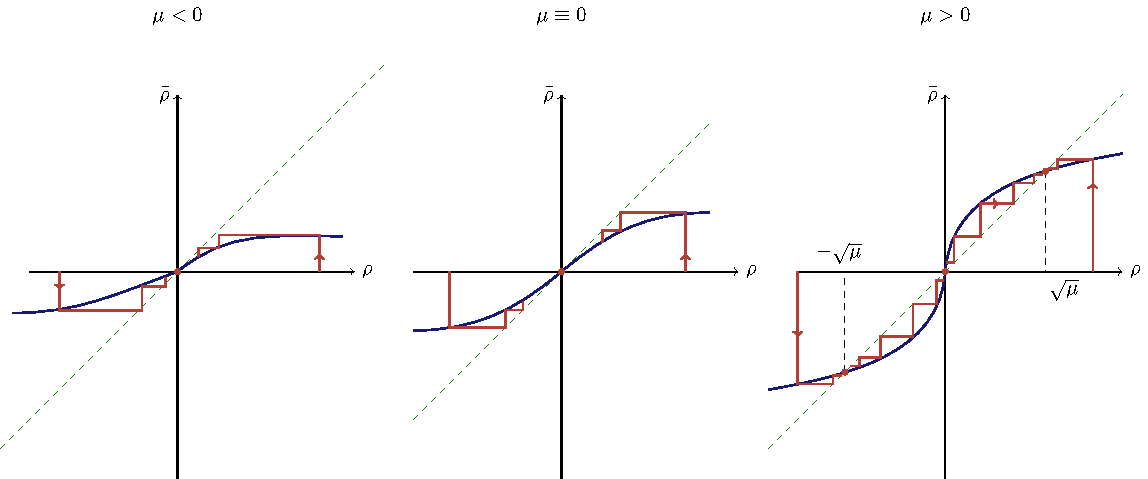
\includegraphics[width=1\linewidth]{fig/fig73.pdf}   
\end{figure}
\begin{figure}[H]
	\centering
	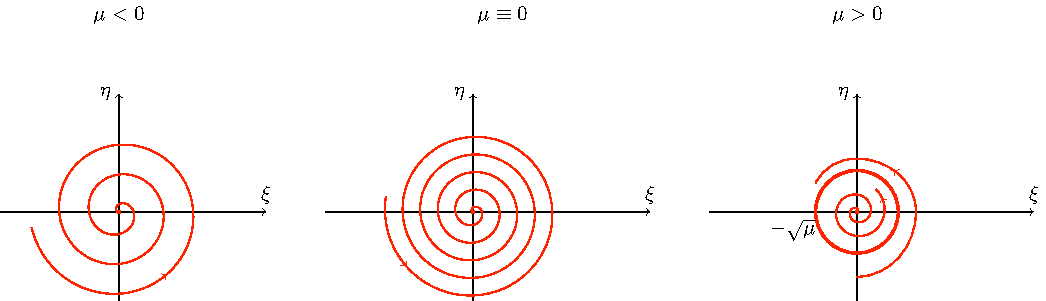
\includegraphics[width=1\linewidth]{fig/fig72.pdf}   
\end{figure}
Справа $\rho \downarrow: ~\stackrel{\_}{\theta}= \theta+\omega$ -- неподвижная точка, преобразование поворота на угол $\omega$. По середине -- то же самое, характер подхода другой. Справа -- есть замкнутая инвариантная кривая радиуса $\sqrt{\mu}$.
Правильно рисовать не сплошными линиями, а точками, поскольку это не отображение.

\subsection{Бифуркация Неймара-Сакера}
\begin{center}
    \begin{minipage}{0.32\linewidth}
        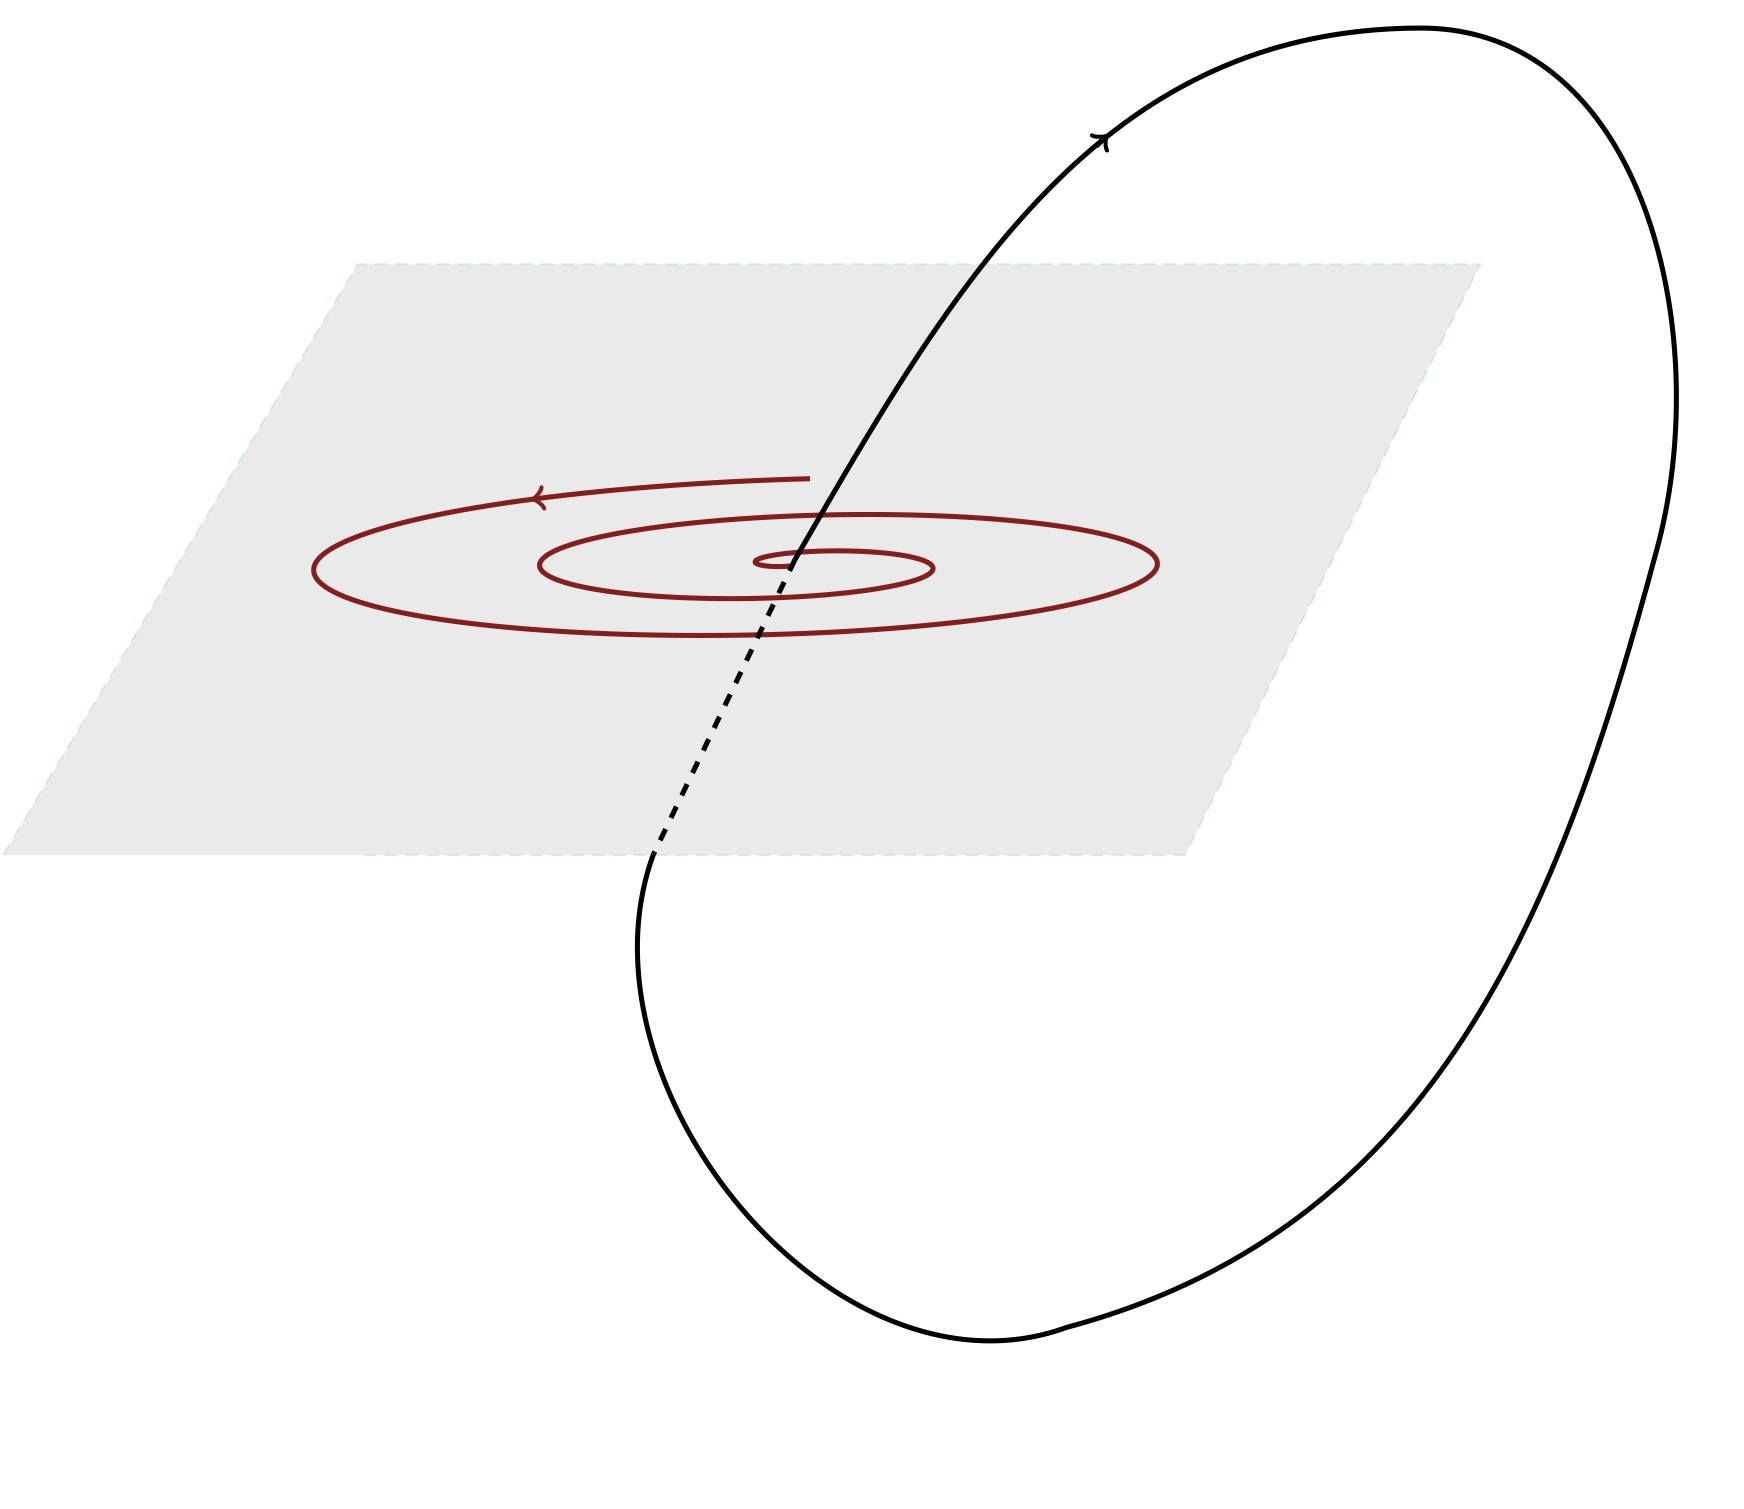
\includegraphics[width=\linewidth]{fig/fig74.jpg} 
        \vspace{-50pt}
        \label{fig:1}
    \end{minipage}
\hfill     
    \begin{minipage}{0.3\linewidth}
        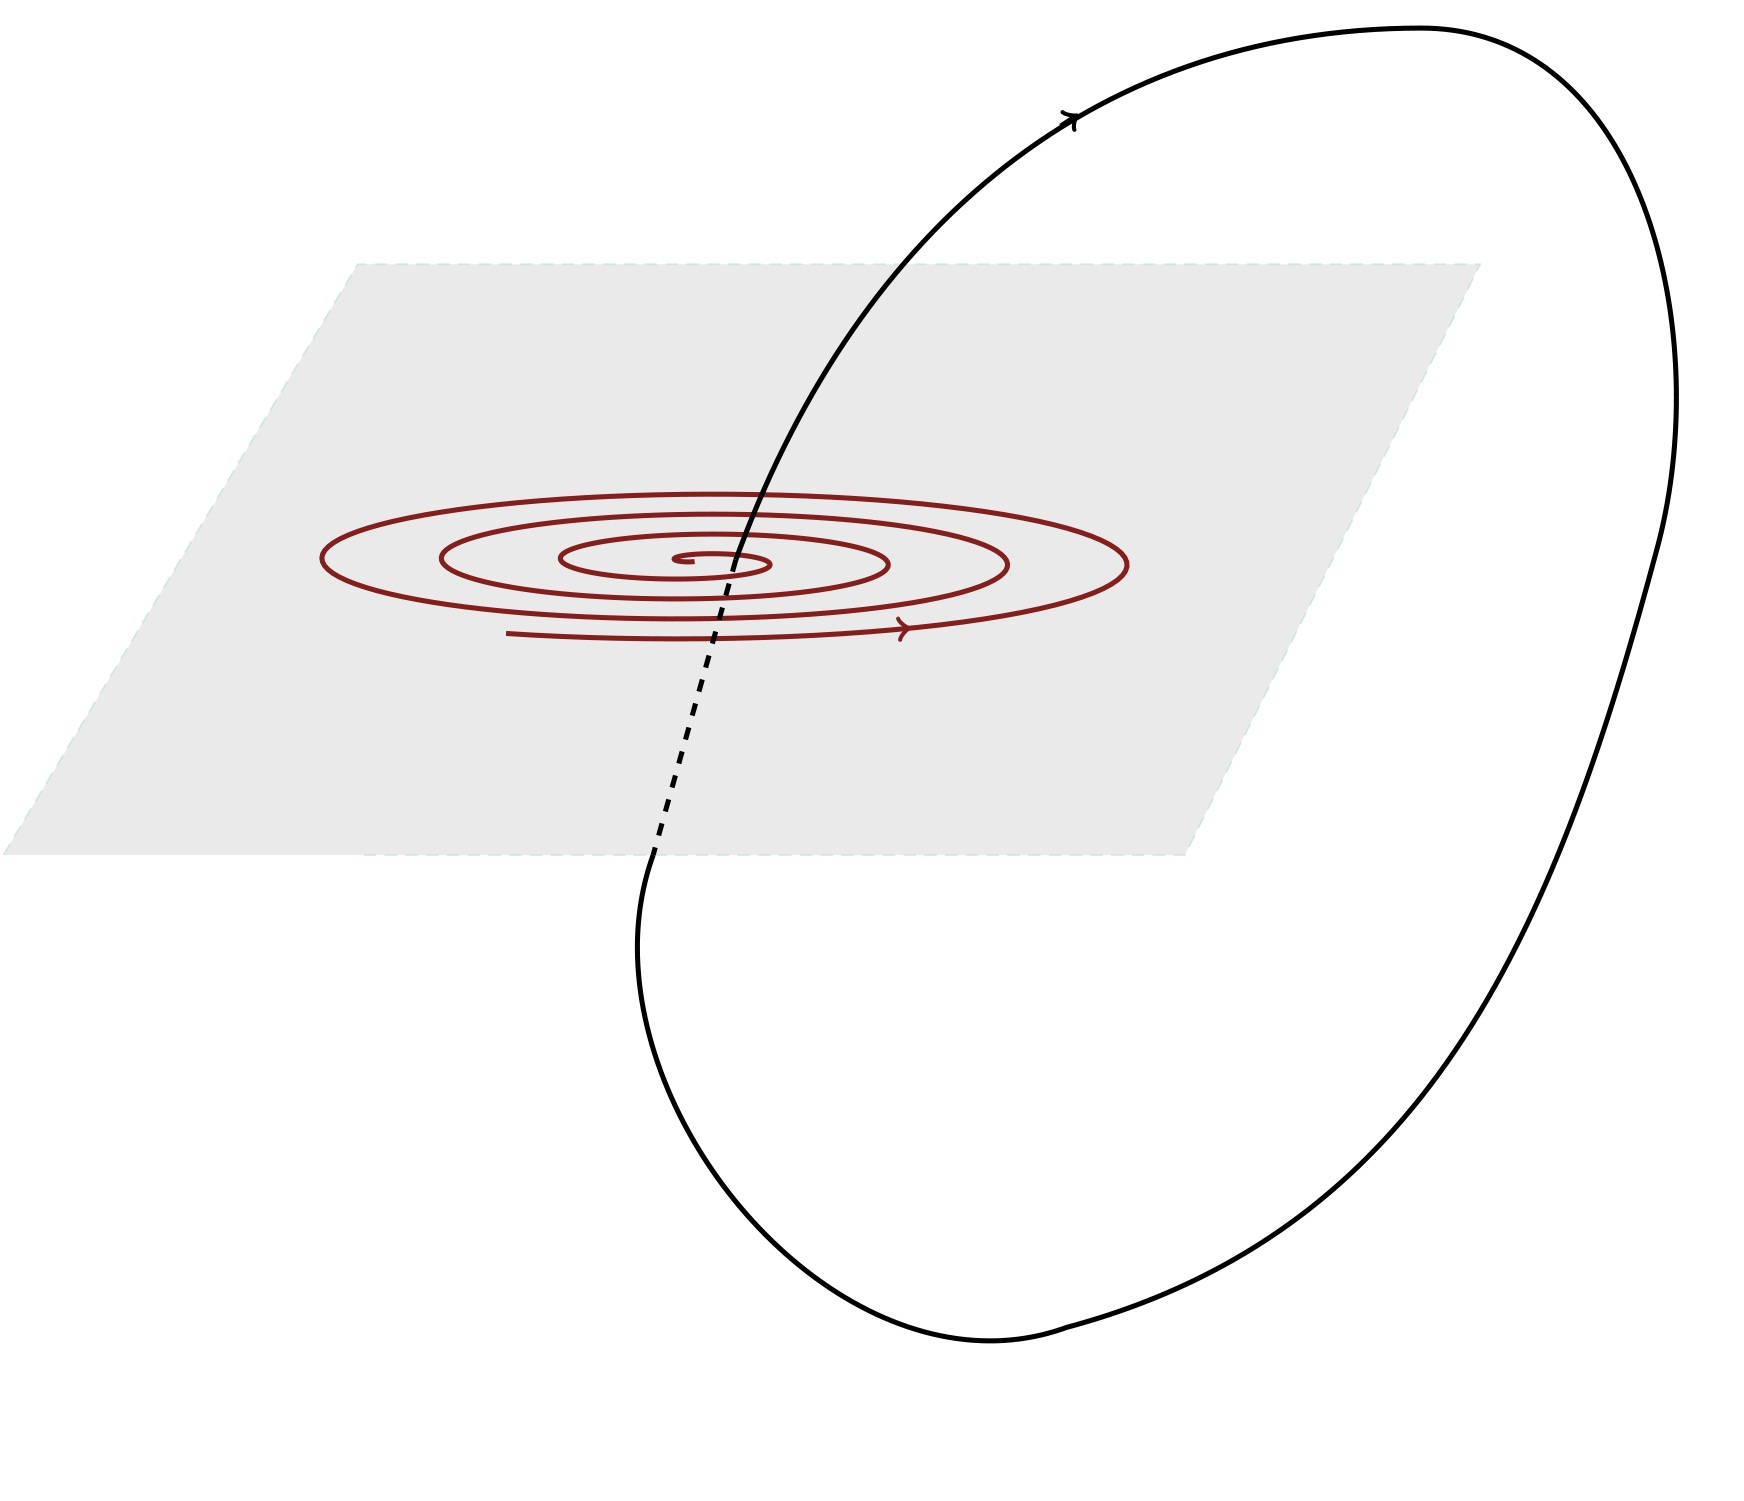
\includegraphics[width=\linewidth]{fig/fig75.jpg} 
        \vspace{-50pt}
        \label{fig:1}
    \end{minipage}
\hfill     
    \begin{minipage}{0.3\linewidth}
        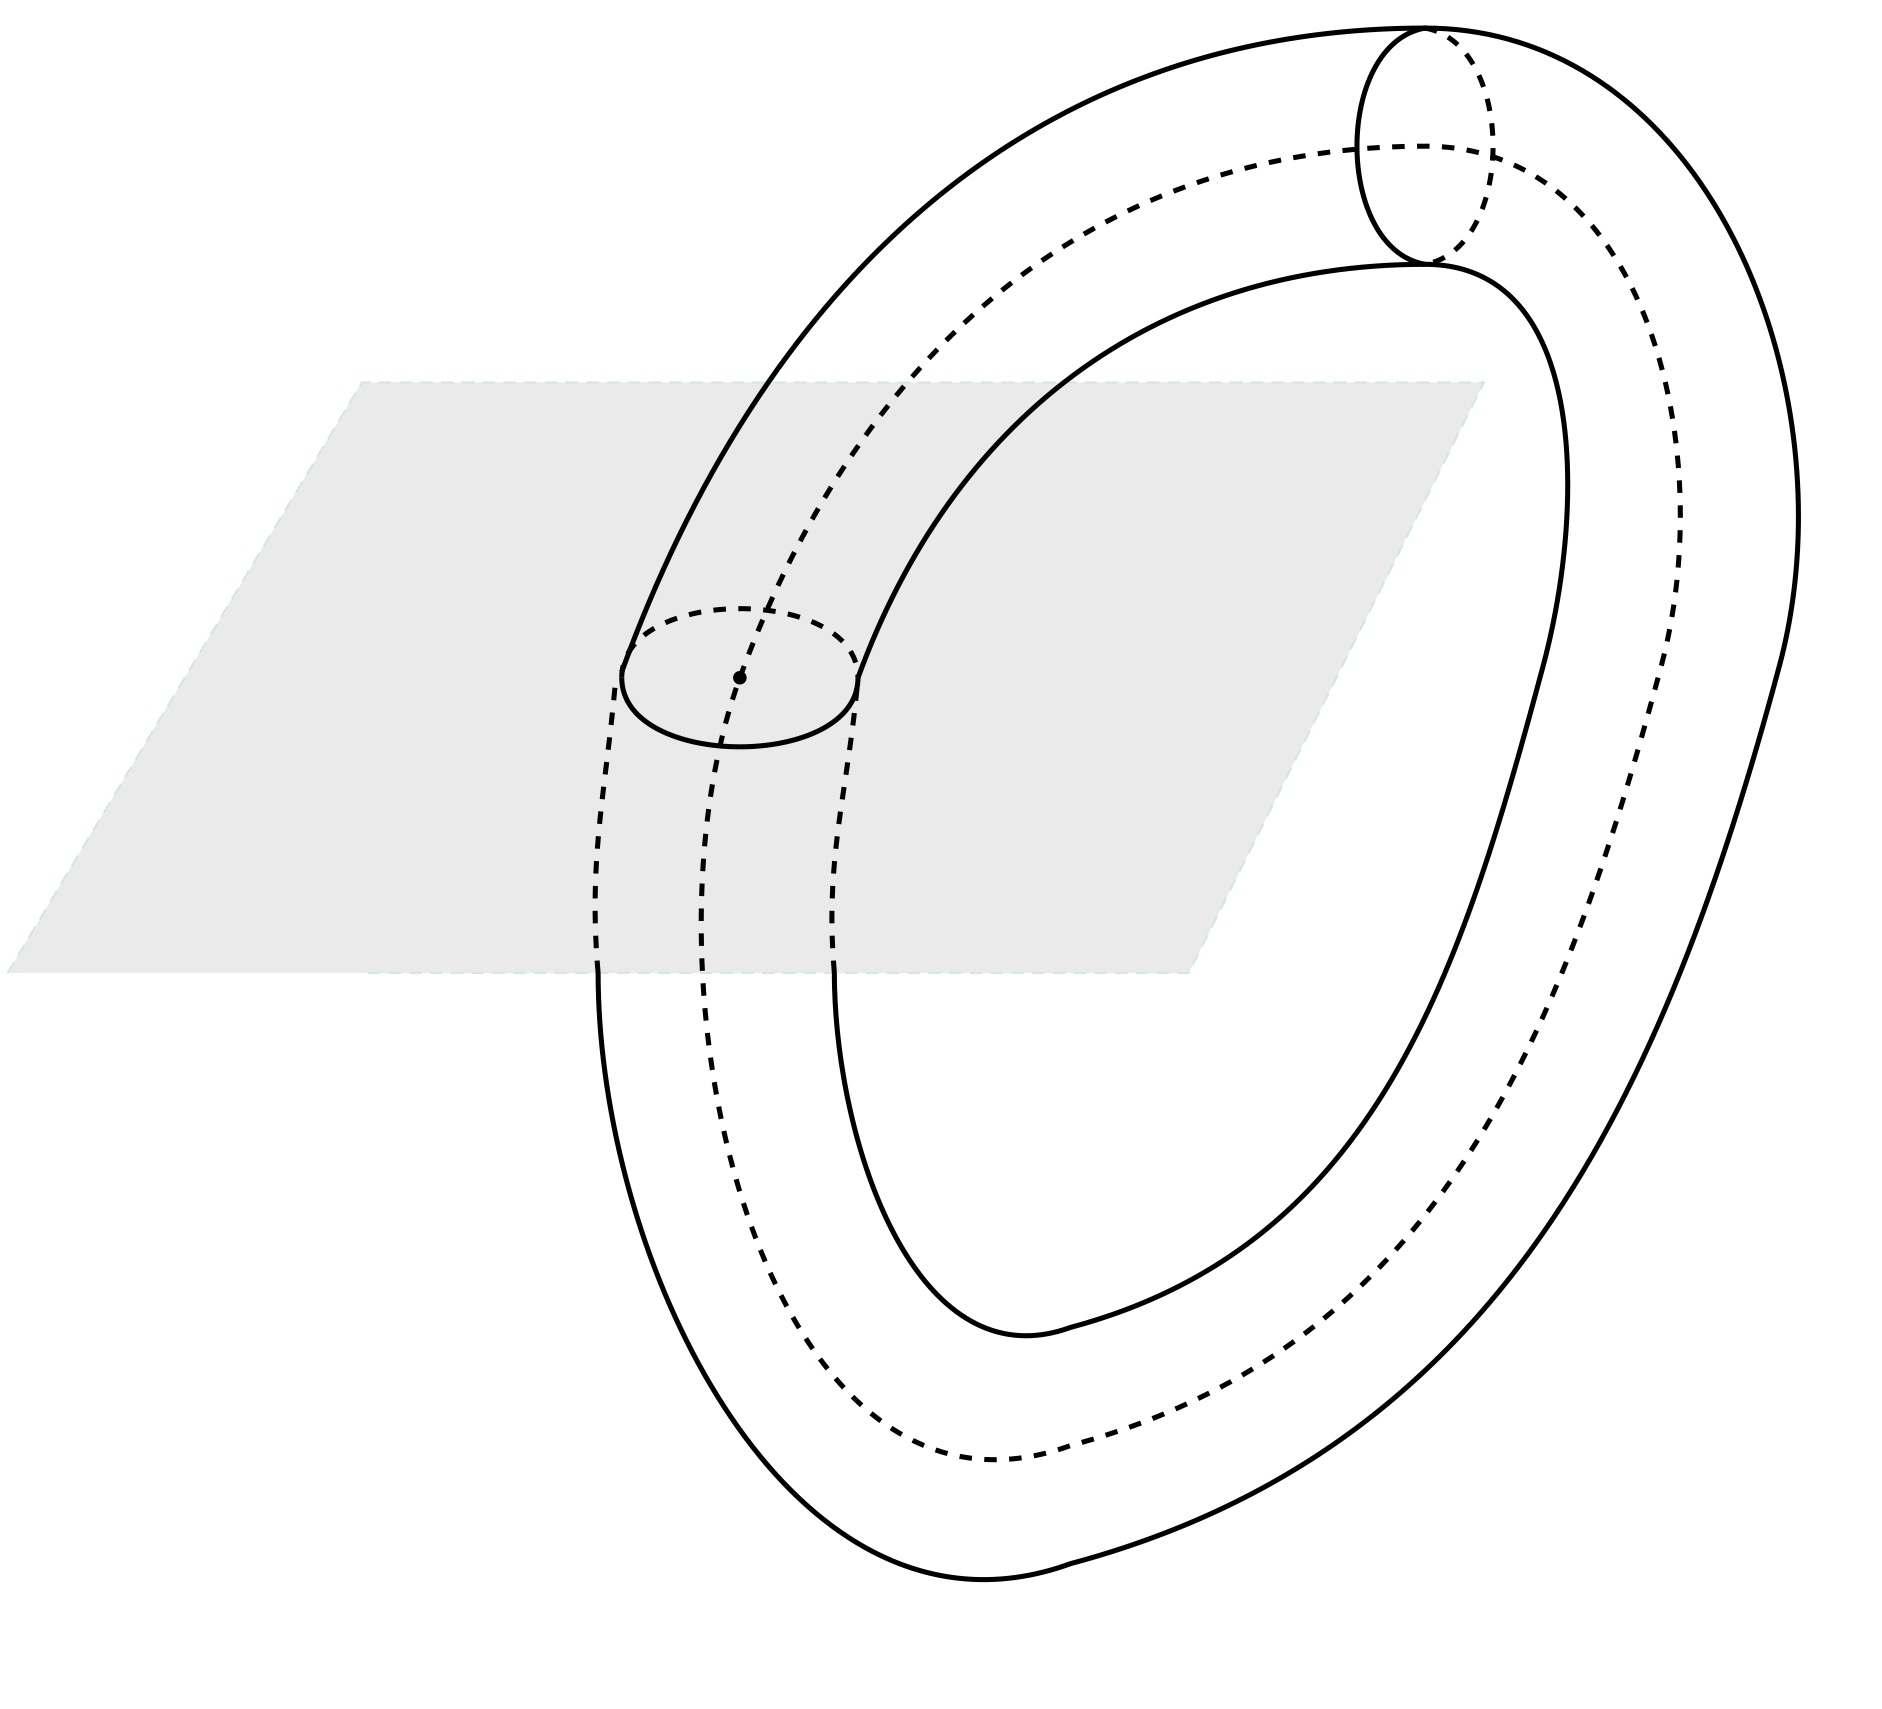
\includegraphics[width=\linewidth]{fig/fig76.jpg} 
        \vspace{-50pt}
        \label{fig:1}
    \end{minipage}    
\end{center}
Слева -- устойчивый предельный цикл. По центру -- то же самое, но с более плотной накруткой. Справа - двумерный инвариантный тор, внутри которого неустойчивый предельный цикл. 

Поведение на торе: либо периодические движения, когда $\frac{\omega_1}{\omega_0}$(одна близка к предельному циклу, другая связана с существованием тора) есть рациональное число. Когда дробь иррациональна движения квазипериодические.